\documentclass[a4paper,12pt]{article}
\usepackage[utf8]{inputenc}
\usepackage[T1]{fontenc}
\usepackage{graphicx}
\usepackage{enumitem}
\usepackage{geometry}
\usepackage{titling}
\usepackage{parskip}
\usepackage[colorlinks=true, allcolors=blue]{hyperref}
\usepackage{array}
\usepackage{booktabs}
\usepackage{listings}
\usepackage{array}
\usepackage{fancyvrb}
\usepackage[table]{xcolor}
\usepackage{hyperref}
\geometry{margin=2.5cm}

\lstdefinestyle{javascript}{
    language=Java,
    basicstyle=\ttfamily\footnotesize,
    keywordstyle=\color{blue},
    commentstyle=\color{green},
    stringstyle=\color{red},
    numbers=left,
    numberstyle=\tiny\color{gray},
    breaklines=true,
    frame=single,
    showspaces=false,
    showstringspaces=false,
    tabsize=2,
    upquote=true,
    columns=fixed,
    basewidth=0.5em
}
\title{Práctica 4: Módulos Odoo Modelo y Vista.}
\author{Andrea Sofía Pais Dos Santos}
\date{\today}

\begin{document}
\setlength{\droptitle}{0.4\textheight} 
\maketitle
\thispagestyle{empty}
\newpage 


\vspace{7cm}

\section{Índice}

\begin{enumerate}[start=2]
    \item Introducción  ....................................................................................... página 3
    \item Actividad 01 - Lista Tareas ................................................................ página 4
    \begin{itemize}
    \item Nueva vista para ver las tareas en formato "Kanban"
    \item Vista visualización "Calendario" según fecha
    \item Errores encontrados
    \end{itemize}
    \item Actividad 02 -  Biblioteca de Cómics .................................................. página 4
    \begin{itemize}
    \item Gestionar socios y atributos
    \item Nuevo modelo para gestionar ejemplares
    \item Restricciones
    \item Errores encontrados 
    \end{itemize}
    \item Actividad 03 ....................................................................................... página 4
    \begin{itemize}
    \item Módulo para gestionar pacientes, médicos y consultas
    \item Implementar las vistas adecuadas para los 3 modelos
    \item Errores encontrados 
    \end{itemize}
    \item Actividad 04 ....................................................................................... página 4
    \begin{itemize}
    \item Crear 4 modelos (Ciclo Formativo, Módulo, Alumno y Profesor)
    \item Implementar los modelos, relaciones y vistas necesarias
    \item Errores encontrados 
    \end{itemize}
    \item Conclusiones ....................................................................................... página 12
\end{enumerate}
\newpage


\section{Introducción}

El objetivo de la práctica es crear y modificar módulos para seguir adquiriendo conceptos y ser capaces de crear módulos por nuestra cuenta


\section{Actividad 01 - Lista Tareas}
El objetivo de la primera actividad es modificar el módulo que creamos en la anterior práctica añadiéndole dos vistas nuevas. La primera una vista Kanban y la segunda una vista que visualiza un Calendario.

\begin{itemize}
    \item Nueva vista en formato Kanban 
    \begin{itemize}
        \item Creamos un nuevo archivo xml "view kanban" que va a tener la siguiente estructura pero un nivel básico para ir entendiendo poco a poco:
        
        \vspace{0.5cm}
        \begin{lstlisting}[style=javascript]
<?xml version="1.0" encoding="utf-8"?>
<odoo>
    <!-- Vista Kanban para la lista de tareas -->
    <record id="lista_tareas_kanban_view" model="ir.ui.view">
        <field name="name">lista_tarea.kanban.view</field>
        <field name="model">lista_tareas.lista_tareas</field>
        <field name="arch" type="xml">
            <!-- Campos necesarios agrupados por el estado que es lo que hace mas agil el estilo kanban-->
            <kanban default_group_by="realizada">
                <field name="tarea"/>
                <field name="categoria"/>
                <field name="prioridad"/>
                <field name="urgente"/>
                <field name="realizada"/>
                
                <!-- Vista de cada tarjeta en la vista Kanban -->
                <templates>
                    <t t-name="kanban-box">
                        <div class="oe_kanban_card oe_kanban_global_click">
                            <!-- Nombre de la tarea -->
                            <strong><field name="tarea"/></strong>
                            <div>
                                <!-- Mostrar la etapa (estado) de la tarea -->
                                <span>Prioridad: <field name="prioridad" /></span><br/>
                            </div>
                        </div>
                    </t>
                </templates>
            </kanban>
        </field>
    </record>
</odoo>
    \end{lstlisting}
    \item Ponemos los campos que tenemos en el modelo del módulo, luego vamos a tener que añadir el del tiempo para el calendario. 
    \item Necesitamos que se vea en otra vista por lo que en la vista principal tenemos que añadir a las acciones kanban.

\vspace{0.5cm}
\begin{lstlisting}[style=javascript]
<field name="view_mode">list,form,kanban</field>
\end{lstlisting}    
    \item Para que el modelo tenga en cuenta al la vista que creamos tenemos que añadir la vista al archivo manifest.

\vspace{0.5cm}
\begin{lstlisting}[style=javascript]
# -*- coding: utf-8 -*-
{
    'name': "Lista de tareas",
    'summary': """Sencilla Lista de tareas""",
    'description': """Sencilla lista de tareas utilizadas para crear un nuevo modulo con un nuevo modelo de datos""",
    'author': "Andrea Sofia Pais Dos Santos",
    'application': True,
    'category': 'Productivity',
    'version': '0.1',
    'depends': ['base'],
    'data': [
        'security/ir.model.access.csv',
        'views/views.xml',
        'views/view_kanban.xml' # -*- hay que poner las vistas que vamos creando -*-
    ],
}
\end{lstlisting} 
    \item Al realizar los cambios lo que tenemos que hacer es actualizar la aplicación que habíamos creado en la otra práctica. Al entrar a la aplicación vemos la vista que principal y ahora vemos una que hay una nueva vista que nos enseña las tareas en formato tarjeta. Las podríamos hacer más bonitas con css, este sería el estilo básico de kanban. Se dividen en dos columnas los que están realizadas y las que no.
    \vspace{0.5cm}

    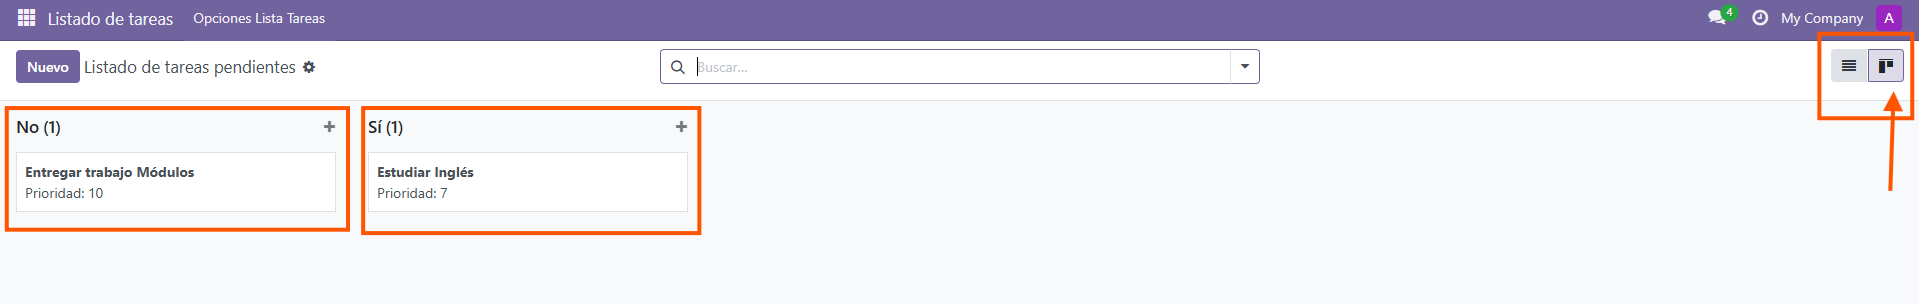
\includegraphics[height=2.3cm]{images/modulo1.png}
    \end{itemize}
    \vspace{0.5cm}

    \item Vista visualización "Calendario" según fecha
    \begin{itemize}
        \item Hay que seguir más o menos los mismos pasos que para hacer la vista kanban. Creamos un archivo para el Calendario, pero lo primero es añadir un atributo nuevo a la vista principal que va a ser la fecha asignada.
        \item En el archivo models vamos a añadir el campo fecha asignada de las tareas que se va a crear.

\vspace{0.8cm}
\begin{lstlisting}[style=javascript]
from odoo import models, fields, api
#Definimos el modelo de datos
class lista_tareas(models.Model):
#Nombre y descripcion del modelo de datos
    _name = 'lista_tareas'
    _description = 'lista_tareas'
    #Elementos de cada fila del modelo de datos
    #Los tipos de datos a usar en el ORM son
    tarea = fields.Char(string="Tarea")
    prioridad = fields.Integer(string="Prioridad")
    urgente = fields.Boolean(compute="_value_urgente", store=True)
    realizada = fields.Boolean(string="Realizada")
    categoria = fields.Selection([
        ("estudio","Estudio"),
        ("trabajo","Trabajo"),
        ("ocio","Ocio"),
        ("cita","Citas")
    ],string="Categoria",default="cita")
    date_deadline= fields.Date(string="Fecha",default=fields.Date.today) # Ponemos el campo fecha que necesitamos para el calendario
    @api.depends('prioridad')
    def _value_urgente(self):
    #Para cada registro
        for record in self:
        #Si la prioridad es mayor que 10, se considera urgente, en otro caso no lo es
            if record.prioridad>10:
                record.urgente = True
            else:
                record.urgente = False
\end{lstlisting} 
    \item Luego en la vista principal añadimos el atributo fecha asignada.
\begin{lstlisting}[style=javascript]
# ... trozo del archivo
<record model="ir.ui.view" id="lista_tareas_form">
      <field name="name">lista_tareas_form</field>
      <field name="model">lista_tareas</field>
      <field name="arch" type="xml">
        <form>
          <sheet>
            <group>
              <group string="La informacion principal">
                <field name="tarea" required="1"/>
                <field name="categoria"/>
                <field name="prioridad"/>
                <field name="date_deadline/> #Ponemos el atributo fecha nuevo
              </group>
              <group string="Estado">
                <field name="realizada"/>
                <field name="urgente"/>
              </group>
            </group>
          </sheet>
        </form>
      </field>
    </record>
...
\end{lstlisting}     
        \item Ahora en el archivo que creamos para la vista Calendario vamos a tener la siguiente estructura:

\vspace{0.5cm}
\begin{lstlisting}[style=javascript]
<?xml version="1.0" encoding="utf-8"?>
<odoo>
    <record id="lista_tareas_calendar_view" model="ir.ui.view">
        <field name="name">lista_tareas.calendar.view</field>
        <field name="model">lista_tareas</field>
        <field name="arch" type="xml">
            <!-- Estructura de la vista calendario-->
            <calendar string="Calendario de Tareas"
                      date_start="date_deadline" 
                      date_stop="date_deadline"
                      color="categoria"
                      mode="month">
                <!-- Campos que se muestran -->
                <field name="tarea"/>
                <field name="prioridad"/>
                <field name="date_deadline"/>
            </calendar>
        </field>
    </record>
</odoo>
\end{lstlisting} 
        \item En el manifest hay que añadir la vista Calendario.
\begin{lstlisting}[style=javascript]
# -*- coding: utf-8 -*-
{
    'name': "Lista de tareas",
    'summary': """Sencilla Lista de tareas""",
    'description': """Sencilla lista de tareas utilizadas para crear un nuevo modulo con un nuevo modelo de datos""",
    'author': "Andrea Sofia Pais Dos Santos",
    'application': True,
    'category': 'Productivity',
    'version': '0.1',
    'depends': ['base'],
    'data': [
        'security/ir.model.access.csv',
        'views/views.xml',
        'views/view_kanban.xml',  # -*- hay que poner las vistas que vamos creando -*-
        'views/view_calendario.xml' # -*- y ahora la vista para el calendario -*-
    ],
}
\end{lstlisting} 
        \item Necesitamos que se vea en otra vista por lo que en la vista principal tenemos que añadir a las acciones el calendario.
\begin{lstlisting}[style=javascript]
<field name="view_mode">list,form,kanban,calendar</field>
\end{lstlisting}    
        \item Al tener todos los archivos bien, actualizamos el módulo vemos que tenemos una nueva vista que nos abre a un calendario mensual que almacena las tareas que vamos añadiendo.
        
        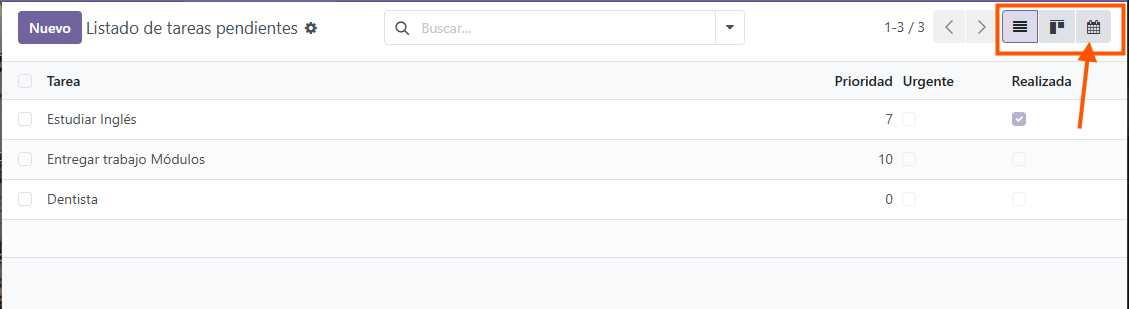
\includegraphics[height=4cm]{images/calendario3.png}

        \item Por ejemplo, vamos a crear una nueva tarea y ahora nos da la opción de seleccionar una fecha en la que ocurrirá la tarea.
        
        \begin{center}
            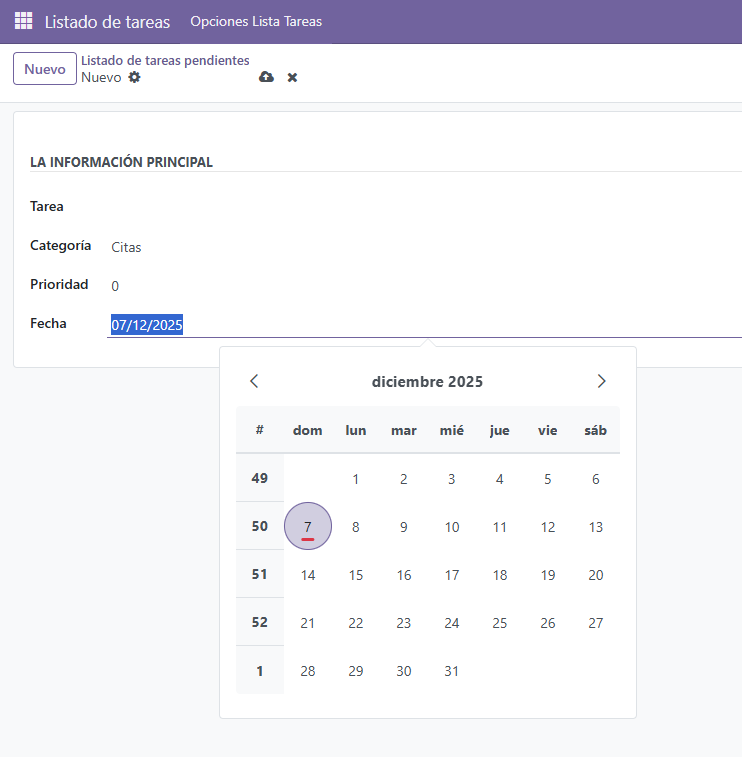
\includegraphics[height=10cm]{images/calendario1.png}
        \end{center}

        \item Ahora, accedemos al calendario y vemos las tareas 
        \begin{center}
            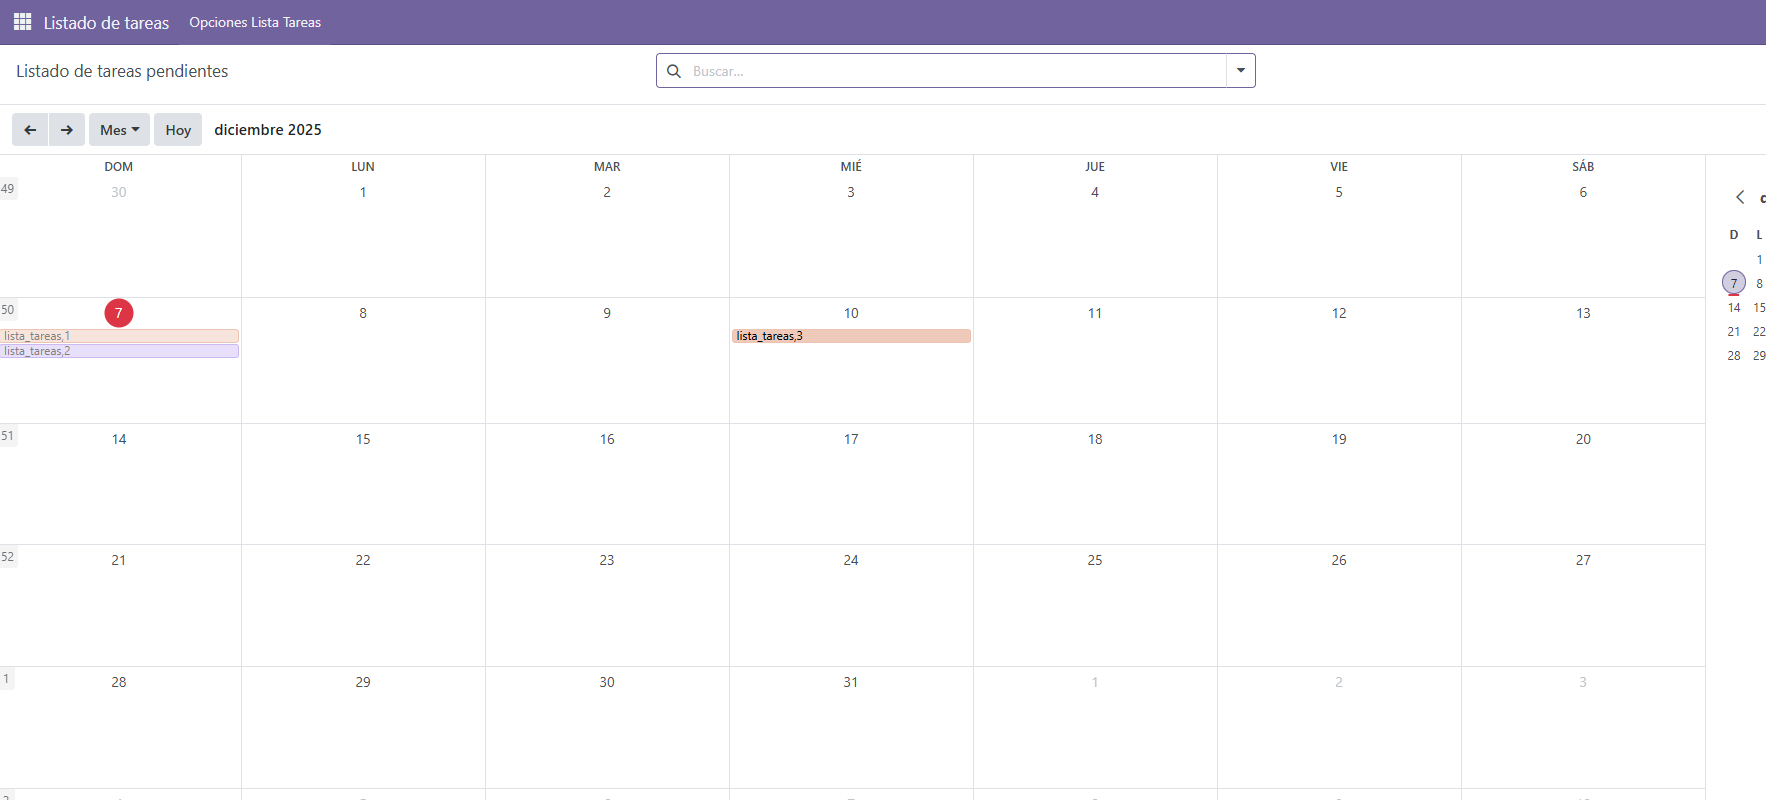
\includegraphics[height=6cm]{images/calendario2.png}
        \end{center}
        \vspace{1.2cm}
        
    \end{itemize}
    \item Errores encontrados
    \begin{itemize}
        \item Tuve un error que no me dejaba actualizar la aplicación de la lista de tareas y era porque me faltaba añadir la lista al manifest.
        \item Un error que tuve al actualizar la aplicación me detectó un error en el nombre del módulo. En esta versión de Odoo, el nombre del modelo debe de ser simplemente el nombre del módulo, no duplicado. Y lo tuve que cambiar en todos los archivos.
        
        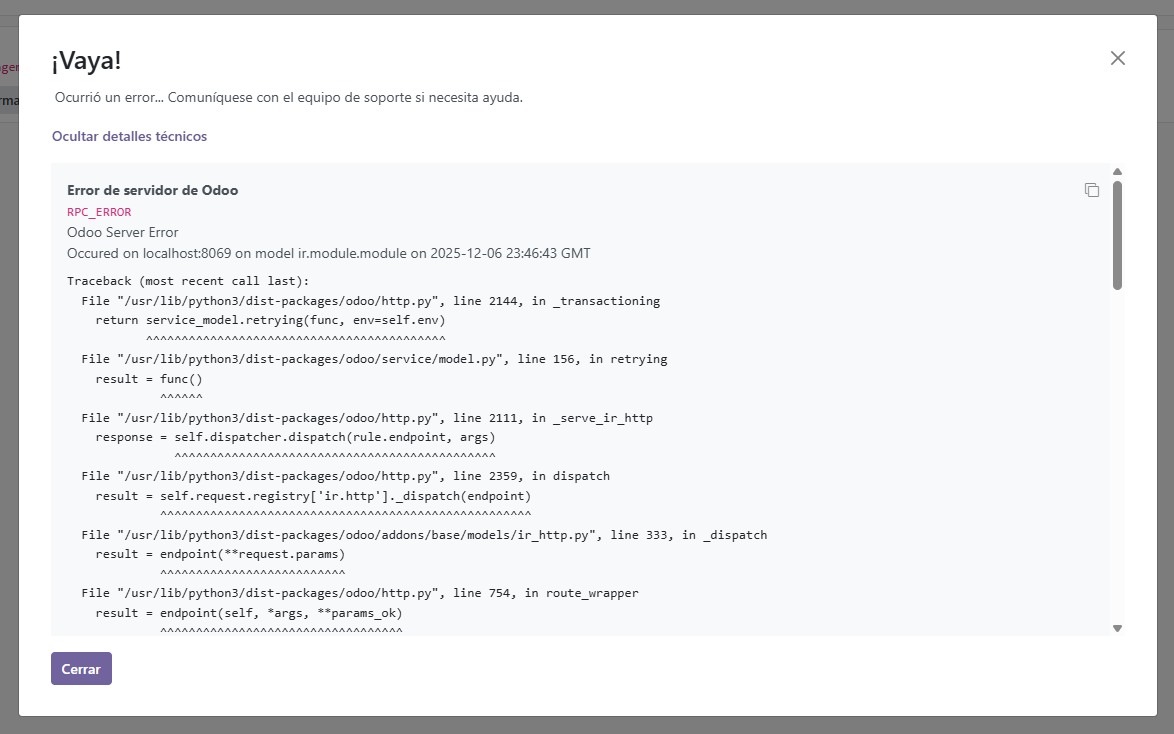
\includegraphics[height=9cm]{images/error1.png}
    \end{itemize}
\end{itemize}

\vspace{1cm}
\section{Actividad 02 -  Biblioteca de Cómics}
El objetivo de la primera actividad 



\section{Actividad 03 -  }
El objetivo de la primera actividad 


\section{Actividad 04 -  }
El objetivo de la primera actividad 

\end{document}